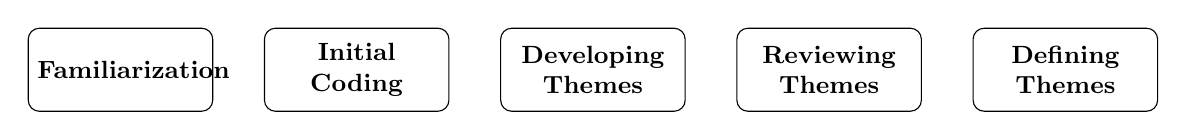
\begin{tikzpicture}[node distance=2cm]
    \definecolor{front-color}{HTML}{ffffff}
    \tikzstyle{every node}=[font=\small]
    \tikzstyle{front} = [rectangle, draw, fill=front-color, text width=6em, text centered, rounded corners, minimum height=3em]
        \node (front1) [front] {\textbf{Familiarization}}; 
        \node (front2) [front, right of=front1, xshift=1cm] {\textbf{Initial Coding}}; 
        \node (front3) [front, right of=front2, xshift=1cm]{\textbf{Developing Themes}}; 
        \node (front4) [front, right of=front3, xshift=1cm]{\textbf{Reviewing Themes}}; 
        \node (front5) [front, right of=front4, xshift=1cm]{\textbf{Defining Themes}}; 
\end{tikzpicture}